% Topic extraction and stance analysis (T2): two tracks and the aggregation to the support share.
% Track 1: hearing summaries -> subjects (04_track1_production) -> clustering (08_taxonomy_consensus)
%          -> drafted labels (09_codebook_draft) -> review and frozen codebook (10_codebook_freeze_assign).
% Track 2: legislator turns (01_member_turns) -> stance records (03_track2_production, 05_assemble)
%          -> placement under the codebook (10_codebook_freeze_assign).
% Track 1 ends with the manual grouping of the 111 topics (T2.4 topic_groups.csv);
% Aggregation: support share by Congress (T2.4.2).
% Same visual language as T3/TEMP/T3.X - Flowchart. Compile: pdflatex fig_topic_extraction_flowchart.tex
\documentclass[border=8pt]{standalone}
\usepackage[T1]{fontenc}
\usepackage{tgtermes}
\usepackage{tikz}
\usetikzlibrary{positioning, shapes.symbols, shadows, arrows.meta, fit, backgrounds, calc}

% Figure Style Guide colors (S3)
\definecolor{RED}{HTML}{B31942}
\definecolor{BLUE}{HTML}{0A3161}
\definecolor{MIDNIGHTBLUE}{HTML}{004953}
\definecolor{GREY}{HTML}{A6A6A8}
\definecolor{BLACK}{HTML}{101820}
\colorlet{SUBTEXT}{GREY!35!BLACK}

% second line inside a block: the fact behind the block, in small dark grey
\newcommand{\sub}[1]{\\[2pt]{\scriptsize\color{SUBTEXT}#1}}

\begin{document}
\hyphenpenalty=10000 \exhyphenpenalty=10000
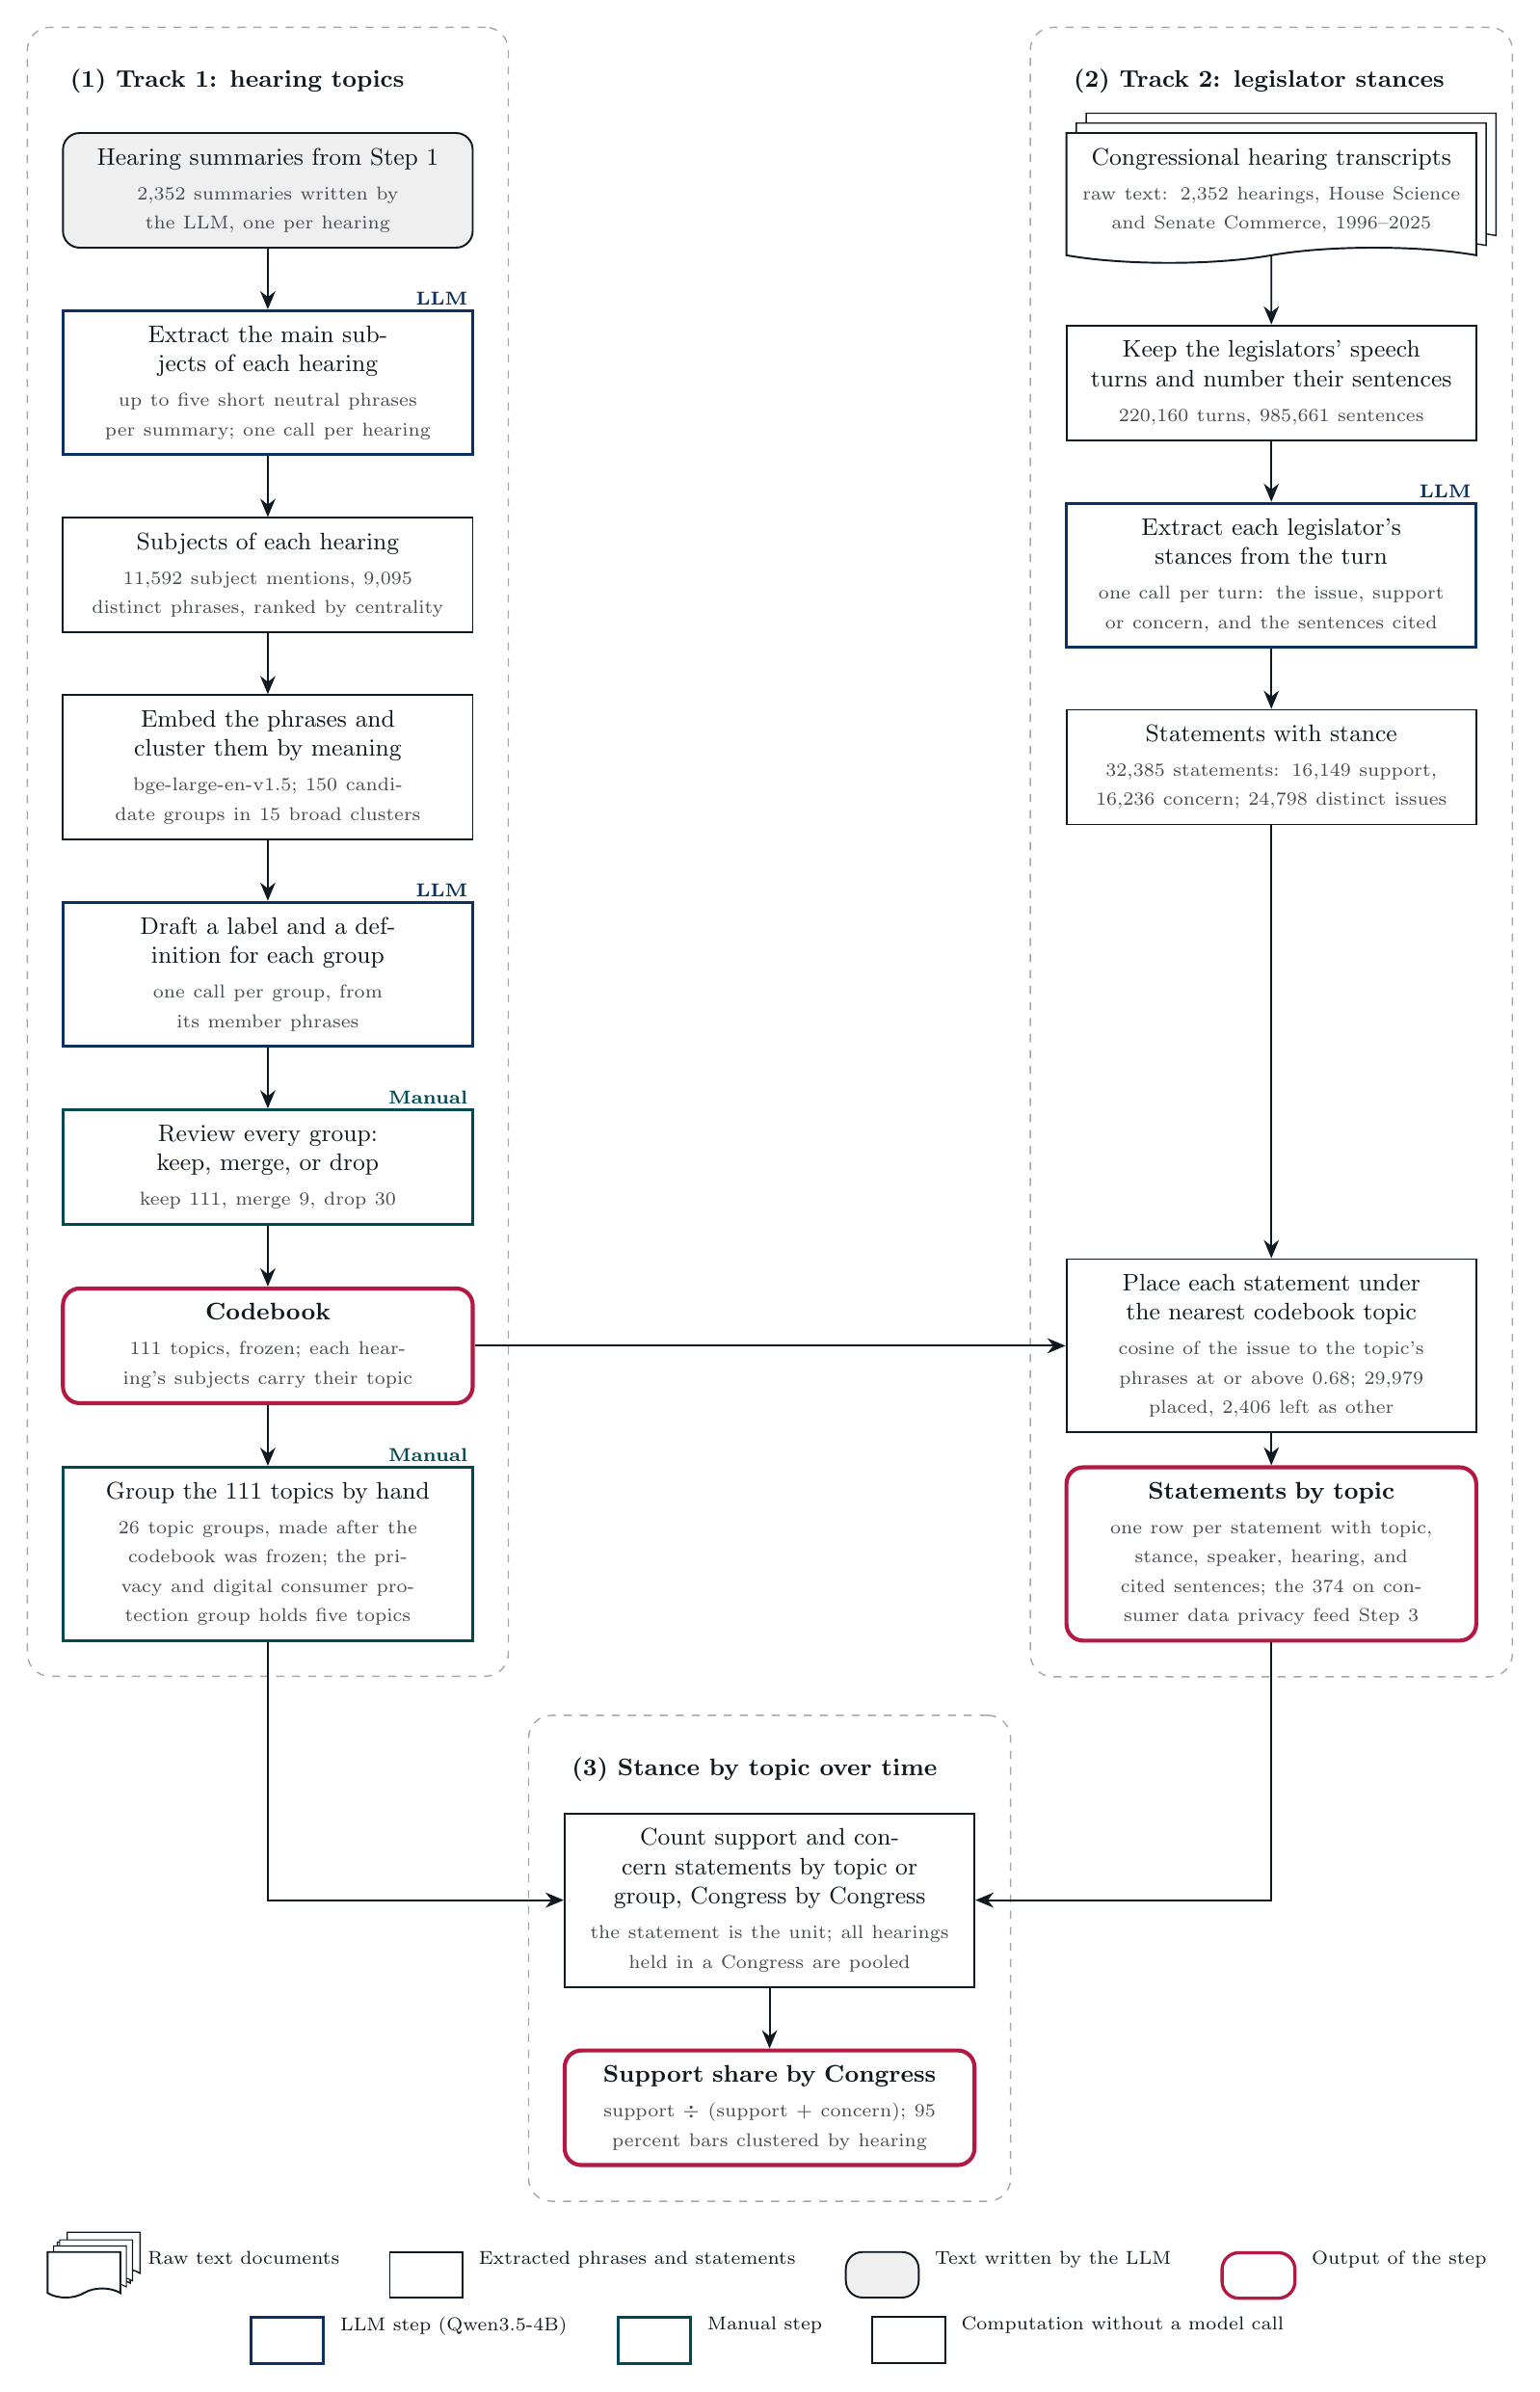
\begin{tikzpicture}[
  font=\small, text=BLACK, color=BLACK,
  node distance=8mm and 14mm,
  every node/.style={align=center},
  flow/.style={-{Stealth[length=2.4mm, width=2mm]}, line width=0.7pt, BLACK},
  % raw text: a stack of documents with a torn lower edge
  rawdoc/.style={tape, tape bend top=none, tape bend height=2mm, draw=BLACK, line width=0.7pt, fill=white,
                 text width=50mm, minimum height=15mm, inner sep=2mm,
                 double copy shadow={shadow xshift=1.3mm, shadow yshift=1.3mm, draw=BLACK, fill=white, line width=0.5pt}},
  % extracted phrases and statements: lines of text with a bar at the left, as quoted lines
  statements/.style={rectangle, draw=BLACK, line width=0.7pt, fill=white, text width=50mm, minimum height=15mm, inner sep=2mm,
                 append after command={\pgfextra{\draw[BLACK, line width=2.4pt]
                   ($(\tikzlastnode.north west)+(1.3mm,-1.3mm)$) -- ($(\tikzlastnode.south west)+(1.3mm,1.3mm)$);}}},
  % text written by the LLM: rounded, shaded
  summary/.style={rectangle, rounded corners=2.2mm, draw=BLACK, line width=0.7pt, fill=GREY!18,
                  text width=50mm, minimum height=13mm, inner sep=2mm},
  % LLM step: process box in BLUE with an LLM tag
  llm/.style={rectangle, draw=BLUE, line width=1.1pt, fill=white, text width=50mm, minimum height=13mm, inner sep=2mm,
              label={[text=BLUE, font=\scriptsize\bfseries, anchor=south east, inner sep=0pt, xshift=-0.8mm, yshift=0.5mm]north east:LLM}},
  % manual step: process box in MIDNIGHT BLUE with a Manual tag
  manual/.style={rectangle, draw=MIDNIGHTBLUE, line width=1.1pt, fill=white, text width=50mm, minimum height=13mm, inner sep=2mm,
              label={[text=MIDNIGHTBLUE, font=\scriptsize\bfseries, anchor=south east, inner sep=0pt, xshift=-0.8mm, yshift=0.5mm]north east:Manual}},
  % computation without a model call
  compute/.style={rectangle, draw=BLACK, line width=0.7pt, fill=white, text width=50mm, minimum height=13mm, inner sep=2mm},
  % data products of the step
  output/.style={rectangle, rounded corners=2.2mm, draw=RED, line width=1.5pt, fill=white, text width=50mm, minimum height=13mm, inner sep=2mm},
  lane/.style={draw=GREY, line width=0.5pt, dashed, rounded corners=3mm, inner sep=4.5mm},
  lanetitle/.style={font=\small\bfseries, text=BLACK, anchor=south west, inner sep=1mm},
]

% ---------------------------------------------------------------- (1) Track 1: hearing topics and the codebook
\node[summary, minimum height=15mm] (T1) {Hearing summaries from Step 1\sub{2,352 summaries written by the LLM, one per hearing}};
\node[llm, below=of T1] (T2) {Extract the main subjects of each hearing\sub{up to five short neutral phrases per summary; one call per hearing}};
\node[statements, below=of T2] (T3) {Subjects of each hearing\sub{11,592 subject mentions, 9,095 distinct phrases, ranked by centrality}};
\node[compute, below=of T3] (T4) {Embed the phrases and cluster them by meaning\sub{bge-large-en-v1.5; 150 candidate groups in 15 broad clusters}};
\node[llm, below=of T4] (T5) {Draft a label and a definition for each group\sub{one call per group, from its member phrases}};
\node[manual, below=of T5] (T6) {Review every group: keep, merge, or drop\sub{keep 111, merge 9, drop 30}};
\node[output, below=of T6] (T7) {\textbf{Codebook}\sub{111 topics, frozen; each hearing's subjects carry their topic}};
\node[manual, below=of T7, minimum height=18mm] (T8) {Group the 111 topics by hand\sub{26 topic groups, made after the codebook was frozen; the privacy and digital consumer protection group holds five topics}};

% ---------------------------------------------------------------- (2) Track 2: legislator statements with stance
\node[rawdoc, right=78mm of T1] (F1) {Congressional hearing transcripts\sub{raw text: 2,352 hearings, House Science and Senate Commerce, 1996--2025}};
\node[compute] (F2) at (T2 -| F1) {Keep the legislators' speech turns and number their sentences\sub{220,160 turns, 985,661 sentences}};
\node[llm] (F3) at (T3 -| F1) {Extract each legislator's stances from the turn\sub{one call per turn: the issue, support or concern, and the sentences cited}};
\node[statements] (F4) at (T4 -| F1) {Statements with stance\sub{32,385 statements: 16,149 support, 16,236 concern; 24,798 distinct issues}};
\node[compute] (F7) at (T7 -| F1) {Place each statement under the nearest codebook topic\sub{cosine of the issue to the topic's phrases at or above 0.68; 29,979 placed, 2,406 left as other}};
\node[output, minimum height=18mm] (F8) at (T8 -| F1) {\textbf{Statements by topic}\sub{one row per statement with topic, stance, speaker, hearing, and cited sentences; the 374 on consumer data privacy feed Step 3}};

% ---------------------------------------------------------------- (3) stance by topic over time
\coordinate (M) at ($(T1)!0.5!(F1)$);
\node[compute] (B) at ($(T8.south -| M)+(0,-34mm)$) {Count support and concern statements by topic or group, Congress by Congress\sub{the statement is the unit; all hearings held in a Congress are pooled}};
\node[output, below=of B] (C) {\textbf{Support share by Congress}\sub{support ÷ (support + concern); 95 percent bars clustered by hearing}};

% ---------------------------------------------------------------- flows
\draw[flow] (T1) -- (T2);
\draw[flow] (T2) -- (T3);
\draw[flow] (T3) -- (T4);
\draw[flow] (T4) -- (T5);
\draw[flow] (T5) -- (T6);
\draw[flow] (T6) -- (T7);
\draw[flow] (T7) -- (T8);
\draw[flow] (F1) -- (F2);
\draw[flow] (F2) -- (F3);
\draw[flow] (F3) -- (F4);
\draw[flow] (F4) -- (F7);
\draw[flow] (F7) -- (F8);
\draw[flow] (T7) -- (F7);
\draw[flow] (T8.south) |- (B.west);
\draw[flow] (F8.south) |- (B.east);
\draw[flow] (B) -- (C);

% ---------------------------------------------------------------- lanes and titles
\node[lanetitle] (titleT) at ([yshift=4mm]T1.north west) {(1) Track 1: hearing topics};
\node[lanetitle] (titleF) at ([yshift=4mm]F1.north west) {(2) Track 2: legislator stances};
\node[lanetitle] (titleC) at ([yshift=3mm]B.north west) {(3) Stance by topic over time};
\begin{scope}[on background layer]
  \node[lane, fit=(titleT)(T1)(T8)] {};
  \node[lane, fit=(titleF)(F1)(F8)] {};
  \node[lane, fit=(titleC)(B)(C)] {};
\end{scope}

% ---------------------------------------------------------------- legend
% Two matrix nodes, each anchored at the midpoint between the two lanes, so each legend row is centered under them.
\matrix[anchor=north, inner sep=0pt, column sep=1.2mm, row sep=0pt, nodes={inner xsep=0.8mm}] (legend1) at ($(C.south -| M)+(0,-11mm)$) {
  \node[rawdoc, text width=8mm, minimum height=6mm, inner sep=0.8mm, tape bend height=1.2mm,
        double copy shadow={shadow xshift=0.8mm, shadow yshift=0.8mm, draw=BLACK, fill=white, line width=0.4pt}] {}; &[1.5mm]
  \node[font=\scriptsize] {Raw text documents}; &[4.5mm]
  \node[statements, text width=8mm, minimum height=6mm, inner sep=0.8mm] {}; &
  \node[font=\scriptsize] {Extracted phrases and statements}; &[4.5mm]
  \node[summary, text width=8mm, minimum height=6mm, inner sep=0.8mm] {}; &
  \node[font=\scriptsize] {Text written by the LLM}; &[4.5mm]
  \node[output, text width=8mm, minimum height=6mm, inner sep=0.8mm, line width=1.2pt] {}; &
  \node[font=\scriptsize] {Output of the step}; \\
};
\matrix[anchor=north, inner sep=0pt, column sep=1.2mm, row sep=0pt, nodes={inner xsep=0.8mm}] (legend2) at ([yshift=-2mm]legend1.south) {
  \node[rectangle, draw=BLUE, line width=1.1pt, fill=white, text width=8mm, minimum height=6mm, inner sep=0.8mm] {}; &
  \node[font=\scriptsize] {LLM step (Qwen3.5-4B)}; &[4.5mm]
  \node[rectangle, draw=MIDNIGHTBLUE, line width=1.1pt, fill=white, text width=8mm, minimum height=6mm, inner sep=0.8mm] {}; &
  \node[font=\scriptsize] {Manual step}; &[4.5mm]
  \node[compute, text width=8mm, minimum height=6mm, inner sep=0.8mm] {}; &
  \node[font=\scriptsize] {Computation without a model call}; \\
};

\end{tikzpicture}
\end{document}
